%     AMS-LaTeX v.2 template for use with amsart
%
%     Remove any commented or uncommented macros you do not use.
\documentclass{amsart}
%\usepackage[notref,notcite]{showkeys}
\usepackage{extarrows}
\usepackage{tikz-cd}
\usetikzlibrary{matrix}


\newtheorem{theorem}{Theorem}[section]
\newtheorem*{theorem*}{Theorem}
\newtheorem{lemma}[theorem]{Lemma}
 \newtheorem{corollary}[theorem]{Corollary}
 \newtheorem{proposition}[theorem]{Proposition}
 \newtheorem*{mainthm*}{Main Theorem}

\theoremstyle{definition}
\newtheorem{definition}[theorem]{Definition}
\newtheorem{example}[theorem]{Example}
\newtheorem{xca}[theorem]{Exercise}
\newtheorem{observation}[theorem]{Observation}
\newtheorem{conjecture}[theorem]{Conjecture}
\newtheorem{open}{Open Problem}

\theoremstyle{remark}
\newtheorem{remark}[theorem]{Remark}

%\numberwithin{equation}{section}

%    Absolute value notation

\begin{document}

\title[Measure Concentration]{Monotonicity formula and measure concentration for compact minimal submanifolds of the Sphere}



%    Remove any unused author tags.

%    author one information

%    author two information
\author{Vicent Gimeno i Garcia}
\address{Department of Mathematics, Universitat Jaume I-IMAC,   E-12071, 
Castell\'{o}, Spain}
%\curraddr{}
\email{gimenov@mat.uji.es}
\author{Vicente Palmer}
\address{Department of Mathematics, Universitat Jaume I-INIT,   E-12071, 
Castell\'{o}, Spain}
%\curraddr{}
\email{palmer@mat.uji.es}

\thanks{Research partially supported by  the Universitat Jaume I Research Program Project P1-1B2012-18, and DGI-MINECO grant (FEDER) MTM2013-48371-C2-2-PDGI from Ministerio de Ciencia e Inovaci\'{o}n (MCINN), Spain.}


\subjclass[2010]{Primary 58C40, 35P15, (53A10)}

\keywords{volume growth, measure concentration, isometric immersion, mean curvature, minimal submanifold}

%\date{\today}

\dedicatory{}



%%%%%%%%%%%%%%%%%%
%Abstract
%%%%%%%%%%%%%%%%%%%%
\begin{abstract}
To be done. v9\end{abstract}

\maketitle

%%%%%%%%%%%%%%%%%%
%Section: Introduction
%%%%%%%%%%%%%%%%%%%%
\section{Introduction}\label{sec:intro}\
%%%%%%%%%%%%%%%%%%%%%%
Consider a complete $n$-dimensional manifold $\Sigma$ properly and minimally immersed in the Euclidean space $\mathbb{R}^N$ by the function $\varphi:\Sigma\to \mathbb{R}^N$. The comparison formula for the volume of extrinsic balls and extrinsic spheres (for example, see \cite{CLY1984}) states that:
$$
{\rm vol}(D_R(o))\geq {\rm vol}(B_R^{n,0})\quad {\rm and}\quad {\rm vol}(\partial D_R(o))\geq {\rm vol}(\partial B_R^{n,0}).
$$
Here, $o$ is a point of $\varphi(\Sigma)$, $D_R(p)$ is the extrinsic ball of radius $R$ centered at $o$, defined as
$$
D_R(o):=\left\lbrace q\in \Sigma\, :\, {\rm dist}_{\mathbb{R}^N}(o, \varphi(p))<R\right\rbrace,
$$
and $B_R^{n,0}$ is the metric ball of radius $R$ in $\mathbb{R}^n$. The set $D_R(o)$ is the $R$-sublevel set of the restriction of the distance function ${\rm dist}_{\mathbb{R}^N}(o,\cdot)$ to $\Sigma$ via the immersion.
Furthermore, according to the classical monotonicity formula (see, for example, \cite{Simon}, \cite{Meeks2011325}, and \cite{Tkachev1994313}), the function
$$
t\mapsto \frac{{\rm vol}(D_R(o))}{{\rm vol}(B_R^{n,0})}
$$
is non-decreasing.

A similar result can be stated for proper minimal immersions $\varphi:\Sigma\to \mathbb{H}^N(-1)$ into the simply connected Hyperbolic space of constant sectional curvature $-1$, as shown in \cite{Anderson1982477}. Specifically, we have that
$$
{\rm vol}(D_R(o))\geq {\rm vol}(B_R^{n,-1}),\quad  {\rm vol}(\partial D_R(o))\geq {\rm vol}(\partial B_R^{n,-1}),
$$
where $o\in \varphi(\Sigma)$. Additionally, the function
$$
t\mapsto \frac{{\rm vol}(D_R(o))}{{\rm vol}(B_R^{n,-1})}
$$
is non-decreasing. Here, $D_R(o)$ is the extrinsic ball, defined as the $R$-sublevel set of the restriction of the distance function ${\rm dist}_{\mathbb{H}^N(-1)}$ to $\Sigma$, and $B_R^{n,-1}$ is the metric ball of radius $R$ in the Hyperbolic space $\mathbb{H}^{n}(-1)$.

In \cite{Palmer1999607}, the second author extended these results to proper and minimal immersions into Cartan-Hadamard ambient spaces. Other extensions of the comparison for the volume of extrinsic balls and the monotonicity formula in different settings can be found in \cite{Lima20161035} and references therein.

Consider the minimal immersion $\varphi: \Sigma\to \mathbb{S}^N$ of a closed n-dimensional manifold $\Sigma$ into the sphere $\mathbb{S}^N$ of constant sectional curvature $1$. In the classic paper by Cheng, Li and Yau \cite{CLY1984}, a mean value inequality for the extrinsic spheres showed that for $0\leq R\leq \frac{\pi}{2}$, the volume of the boundary of the extrinsic ball $D_R(o)$ (defined as the $R$-sublevel set of the distance function ${\rm dist}_{\mathbb{S}^N}$ to $\Sigma$ at a point $o\in \varphi(\Sigma)$) is greater than or equal to the volume of the metric ball $B_R^{n,1}$ of radius $R$ in the sphere $\mathbb{S}^n$, \emph{i.e.},
$$
{\rm vol}(\partial D_R(o))\geq {\rm vol}(\partial B_R^{n,1})\quad {\rm for}\quad 0\leq R\leq \frac{\pi}{2},
$$
Using an inequality for the Neumann eigenvalues of $D_R(o)$, the paper shows that for $0\leq R\leq \pi$, the volume of $D_R(o)$ is greater than or equal to the volume of $B_R^{n,1}$.
In \cite{Markvorsen2002101}, it was proven that the equality is achieved in the above inequality for some $R\in(0,\pi)$ if and only if $\varphi:\Sigma\to \mathbb{S}^N$ is a totally geodesic immersion, implying that $\Sigma$ is isometric to $\mathbb{S}^N$. There is no clear monotonicity formula in this case, but in \cite{Palmer1999607, Markvorsen2002101}, it is proven that the function
$$
t\mapsto \frac{{\rm vol}(D_t(o))-{\rm vol}( B_t^{n,1})}{{\rm vol}(\partial  B_t^{n+1,1})}
$$
is non-decreasing for $t$ in $(0,\pi/2)$, and in \cite{Kokarev2021}, it is proven that the function
$$
t\mapsto \frac{{\rm vol}(D_t(o))}{{\rm vol}(\partial  B_t^{n+1,1})}
$$
is non-decreasing for $t$ in the whole interval $(0,\pi)$.

Considering compact and minimal immersions in the sphere $\mathbb{S}^N$, a natural question arises: for an isometric and minimal immersion $\varphi: \Sigma \to \mathbb{S}^N$ of a closed Riemannian $n$-manifold $\Sigma$ into the sphere $\mathbb{S}^N$, can the function
$$t\mapsto \frac{{\rm vol}(D_t(o))}{{\rm vol}( B_t^{n,1})}$$
be non-decreasing in $(0,\pi]$? The answer is that this is only possible if the immersion is totally geodesic, as shown in the following theorem, which is the first result of this paper:
\begin{theorem}\label{teounua}
Let $\varphi:\Sigma\to\mathbb{S}^N$ an isometric and minimal embedding of the closed $n$-manifold $\Sigma$ into the sphere $\mathbb{S}^N$.  Let ${\rm vol}\left(B^{n,1}_t\right)$ be the volume of the metric ball of radius $t$ of $\mathbb{S}^n$.
 Suppose that $o\in \varphi(\Sigma)$.  Then, if the function
 $$
 t\mapsto \frac{{\rm vol}(D_t(o))}{{\rm vol}\left(B^{n,1}_t\right)}
 $$
 is monotone in $(0,\pi)$, \emph{i.e.}, non-increasing or non-decreasing in $(0,\pi)$, then $\Sigma$ is totally geodesic in $\mathbb{S}^N$, and hence $\Sigma$ is isometric to the $n$-dimensional sphere, $$\Sigma\equiv \mathbb{S}^n.$$
\end{theorem}
Additionally, we can enhance the established monotonicity formulas through the following 
\begin{theorem}\label{teodua}
Let $\varphi:\Sigma\to\mathbb{S}^N$ an isometric and minimal immersion of the closed $n$-manifold $\Sigma$ into the sphere $\mathbb{S}^N$.  Let ${\rm vol}\left(B^{n,1}_t\right)$ be the volume of the metric ball of radius $t$ of $\mathbb{S}^n$. Then, the function
 $$
 t\mapsto \frac{{\rm vol}(D_t(o))-{\rm vol}\left(B^{n,1}_t\right)}{{\rm vol}\left( \partial B^{n,1+1}_t\right)}
 $$
 is monotone non-decreasing in $(0,\pi)$.
\end{theorem}

 
The concrete value $R=\pi/2$ is a very special value for the radius of an extrinsic ball or, even more, for the radius of an extrinsic sphere.  Technically, in proposition \ref{prop:critics} we will show that almost every critical point for the extrinsic distance function concentrates at extrinsic distance $\pi/2$. Indeed in section \ref{Clifford} we will analyze the particular case of the Clifford torus surface minimally immersed in $\mathbb{S}^3$. Numerical evidences suggest that the function 
$$
t\mapsto \frac{{\rm vol}(D_t(o))}{{\rm vol}\left(B^{2,1}_t\right)}
$$
is non-decreasing up to $t=\pi/2$.

Beyond, this technical considerations,  we can state that in a compact manifold $\Sigma$ isometrically and minimally immersed into the Sphere $\mathbb{S}^N$, the extrinsic equator (the set of points of $\Sigma$ at extrinsic distance $\pi/2$ of any fixed point) \emph{concentrates} measure.

Given a point $o\in \mathbb{S}^N$, and given an isometric immersion $\varphi:\Sigma\to \mathbb{S}^N$, the \emph{Extrinsic equator} $E(o)$ of $\Sigma$ with respect to $o$ is the set
$$
E(o):=\{ q\in \Sigma\, : \, {\rm dist}_{\mathbb{S}^N}(o,\varphi(q))=\frac{\pi}{2}\} 
$$
When $\varphi:\Sigma\to \mathbb{S}^N$ is an isometric and minimal immersion of the closed manifold $\Sigma$ into the Sphere $\mathbb{S}^N$, by the maximum principle, see proposition \ref{prop:critics}, can be stated that
$$
E(o)\neq \emptyset,
$$
for any $o\in\mathbb{S}^N$. Moreover, the extrinsic $\epsilon$-cousin of $E(o)$ given by
$$
\Omega(p,\epsilon):=\left\lbrace x\in \Sigma\, : \, -\epsilon<\cos({\rm dist}_{\mathbb{S}^N}(o,x))<\epsilon \right\rbrace.
$$
concentrates measure in the sense that the quotient 
$$
\frac{{\rm vol}\left(\Omega(o,\epsilon)\right)}{{\rm vol}(\Sigma)} \to 1\quad {\rm when}\quad {\rm dim}(\Sigma)\to\infty. 
$$
More precisely,
\begin{theorem}\label{teo:conc}
Let $\varphi: \Sigma\to \mathbb{S}^N$ be an isometric and minimal immersion of a closed, (compact and without boundary), $n$-dimensional manifold $\Sigma$ into the sphere  $\mathbb{S}^N$. For any $o\in\mathbb{S}^N$ and for any $\epsilon\in (0,\pi/2)$,  let $\Omega(p,\epsilon)$ be the set
$$
\Omega(o,\epsilon):=\left\lbrace x\in \Sigma\, : \, -\epsilon<\cos({\rm dist}_{\mathbb{S}^N}(o,\varphi(x)))<\epsilon \right\rbrace.
$$
Then,   there exists a constant $C(\epsilon,n)$ depending only on $\epsilon$ and $n$ such that
$$
1-C(\epsilon,n)\leq \frac{{\rm vol}\left(\Omega(o,\epsilon)\right)}{{\rm vol}(\Sigma)}\leq 1.
$$
Moreover,
$$
\lim_{n\to\infty}C(\epsilon,n)=0
$$
\end{theorem}

As a consequence, in the particular case when we consider the trivial, isometric and minimal immersion given by
$$
{\rm id}:\mathbb{S}^N\to \mathbb{S}^N,\quad q\mapsto {\rm id}(q)=q,
$$
we have the classical Vitali-Milman concentration of measure result in the sphere,
\begin{corollary}
Let $\mathbb{S}^N$ be the $N$-dimensional sphere. For any $p\in\mathbb{S}^N$ and for any $\epsilon\in (0,\pi/2)$,  let $\Omega(p,\epsilon)$ be the set
$$
\Omega(p,\epsilon):=\left\lbrace x\in \mathbb{S}^N\, : \, -\epsilon<\cos({\rm dist}_{\mathbb{S}^N}(p,x))<\epsilon \right\rbrace.
$$
Then,   there exists a constant $C(\epsilon,n)$ depending only on $\epsilon$ and $n$ such that
$$
1-C(\epsilon,n)\leq \frac{{\rm vol}\left(\Omega(p,\epsilon)\right)}{{\rm vol}(\mathbb{S}^N)}\leq 1.
$$
Moreover,
$$
\lim_{n\to\infty}C(\epsilon,n)=0
$$
\end{corollary}
%%%%%%%%%%%%%%%%%
% \subsection{Outline}
%%%%%%%%%%%%%%%%%
\subsection{Outline}\

The structure of the paper can be outlined as follows...



\section{Preliminaries}
Given a isometric immersion $\varphi:\Sigma \to \mathbb{S}^N\subset \mathbb{R}^{N+1} $ of the Riemannian $n$-manifold $\Sigma$ into the $N$-sphere
$$
\mathbb{S}^N:=\left\lbrace (x_1,\cdots, x_{N+1})\in \mathbb{R}^{N+1}\, :\, x_1^2+\cdots x_{N+1}^2=1\right\rbrace
$$
Takahashi proved in \cite{Takahashi1966380} that the immersion is minimal if and only if 
\begin{equation}\label{takahashi}
\Delta x_i\circ \varphi=-n x_i\circ \varphi, \quad \text{ for any }\quad i\in \{1,\cdots, N+1\}    
\end{equation}
where $\Delta$ denotes the Riemannian Laplacian of $\Sigma$. To prove our main theorems we are interested in the extrinsic distance function. Given a point $o\in \mathbb{S}^N$ the extrinsic distance function to $o$ is the restriction by $\varphi$ of the distance function ${\rm dist}_{\mathbb{S}^N}$ in $\mathbb{S}^N$ given by
$$
r_o:\Sigma\to \mathbb{R},\quad q\mapsto r_o(q)={\rm dist}_{\mathbb{S}^N}(o,\varphi(q)).
$$
The extrinsic balls and the extrinsic spheres are given therefore by
$$
D_R(o)=\left\lbrace q\in \Sigma\, : r_o(q)<R\right\rbrace, \quad \partial D_R(o)=\left\lbrace q\in \Sigma\, : r_o(q)=R\right\rbrace.
$$
Moreover, the function $\cos\circ r_o$ is a smooth as can be checked in the following expression because
$$
\cos(r_o(q))=\langle o,\varphi(q)\rangle =\sum_{i=1}^{N+1}x_i(o)x_i(\varphi(q)).
$$
and by \eqref{takahashi},
\begin{equation}\label{lapcos}
\Delta\cos(r_o(q))=\sum_{i=1}^{N+1}x_i(o)\Delta x_i(\varphi(q))=-n\cos(r_o(q))    
\end{equation}
Hence, since $r_o$ is a smooth function on $\Sigma-\varphi^{-1}(o)\cup \varphi^{-1}(-o)$,
\begin{equation}\begin{aligned}
-n\cos(r_o(q))=&  {\rm div}(\nabla \cos r_o(o))={\rm div}(-\sin r_o(q)\nabla r_o(q) )\\
=&-\cos(r_o(q))\Vert \nabla r_o(q)\Vert^2-\sin(r_o(q))\Delta (r_o(q)),
\end{aligned}
\end{equation}
for any $q\in \Sigma-\varphi^{-1}(o)\cup \varphi^{-1}(-o)$.
Therefore if $q$ is a critical point of the extrinsic distance function ($\nabla r_o(q)=0$)
\begin{equation}\label{lapcrit}
  n\cos(r_o(q))=\sin(r_o(q))\Delta (r_o(q)). 
\end{equation}
By the maximum principle for parabolic manifolds (in particular, for complete and closed manifolds), see \cite{Alias2016} for instance, we can state the following proposition
\begin{proposition}\label{prop:max}
Let  $\varphi:\Sigma \to \mathbb{S}^N$ be an isometric and minimal  immersion of the complete and parabolic manifold $\Sigma$ into the sphere $\mathbb{S}^N$. Then for any $o\in \mathbb{S}^N$, there are $q_1, q_2\in \Sigma$ such that
$$
r_o(q_1)\leq \frac{\pi}{2}\quad {\rm and}\quad r_o(q_2)\geq \frac{\pi}{2},
$$
and hence there exists $q_3 \in \Sigma$ with $r_o(q_3)=\frac{\pi}{2}$.
\end{proposition}
\begin{proof}
Suppose that $r_o$ is a constant function on $\Sigma$, then $\Vert \nabla r_o\Vert=0=\Delta r_o$ everywhere in $\Sigma$, and by 
equation \eqref{lapcrit}, $\cos r_o(q)=0$ for any $q\in \Sigma$ which implies that $r_o(q)=\frac{\pi}{2}$ for any $q\in \Sigma$. Therefore the proposition follows trivially in this case. 

Suppose otherwise that $r_o$ is non-constant on $\Sigma$, since $\cos r_o$ is bounded, namely,

$$-1\leq u_*:= \inf_\Sigma \cos r_o<\sup_\Sigma \cos r_o=:u^*\leq 1.$$  
Since $\Sigma$ is parabolic, there exist two sequences $\{l_k\}_{k\in\mathbb{N}}\subset \Sigma$ and  $\{u_k\}_{k\in\mathbb{N}}\subset \Sigma$ such that
$$
\cos r_o(l_k)<u_*+\frac{1}{k},\quad \cos r_o(u_k)>u^*-\frac{1}{k},\quad \Delta \cos r_o(l_k)>0, \quad \Delta \cos r_o(u_k)<0.  
$$
Finally the proposition follows by equation \eqref{lapcos}.
\end{proof}
\begin{remark}
Ros \& company.
\end{remark}

Now we are applying  the coarea formula to the function $\psi:=h\circ r_o$ where $h:[0,\pi]\to [0,\pi]$ is the non-decreasing bijection  given by
$$
t\mapsto h(t):=\frac{\pi}{2}-\frac{\pi}{2}\cos(t).
$$
We follow the lines of \cite{Sakai} Chapter II, section 5,  since $\psi$ is a smooth function such that $\psi(\Sigma)=[a,b]$ with $0\leq a<b\leq \pi$ . Denote by $\Omega_0$ the set of critical points of $\psi$. By Sard's theorem, the set of critical values $S_\psi=\psi(\Omega_0)$ has null measure, and the set of regular values $R_\psi=[a,b]-S_\psi$ is open. In particular, for any $t\in R_\psi=[a,b]-S_\psi$, the set $\Gamma(t):=\psi^{-1}(t)$ is a smooth embedded hypersurface in $\Omega$ with $\partial \Gamma(t)=\emptyset$. Since $\Gamma(t)\subseteq\Omega-\Omega_0$ then $\nabla\psi$ does not vanish along $\Gamma(t)$; indeed, a unit normal along $\Gamma(t)$ is given by $\nabla\psi/|\nabla\psi|$. Observe moreover that in this case
$$
\partial D_{t}(o)=\Gamma(h(t)).
$$
Now we let
\begin{equation}
\begin{aligned}
% \Gamma(t) \, &= \, \{ x \in \overline{\Omega} \, \, : \, \,  \psi(x) \, =
% \, t\} \\
 \mathcal{A}(t) \, &= \, {\rm vol}(\Gamma(t))={\rm vol}(\partial D_{h^{-1}(t)}(o) ) \\
\Omega(t) \, &= \,  \{ x \in \overline{\Omega} \, \, | \, \, \psi(x)
 \, <
\, t\} =D_{h^{-1}(t)}(o)\\
\mathcal{V}(t) \, &= \,  \operatorname{Vol}(\Omega(t)) ={\rm vol}(D_{h^{-1}(t)}(p))\quad .
\end{aligned}
\end{equation}

\begin{theorem}\label{thmCoarea}\
\begin{enumerate}

\item Given $g \in L^1(\Sigma, dV)$,

\begin{equation*}
\begin{aligned}
\int_{\Sigma}g\,dV&=\int_{\Omega_0}g\,dV+\int_{\Sigma-\Omega0}(g\,|\nabla\psi|^{-1})\,|\nabla\psi|\,dV\\
\label{eq:coarea}
&=\int_{\Omega_0}g\,dV+\int_{0}^\pi\left(\int_{\Gamma(t)}g\,|\nabla\psi|^{-1}\,dA\right)dt,
\end{aligned}
\end{equation*}
\noindent where $dA$ is the Riemannian volume element defined from the induced metric $g_t$ on $\Gamma(t)$ from $g$.
Where we have used that $S_\psi$ has null measure. 
\item The function $\mathcal{V}(t)$ is a smooth function on the regular values of $\psi$  given by 
\begin{equation*}
  \mathcal{V}(t) \, = \, {\rm vol}(\Omega_0\cap \Omega(t))+\int_a^t\left(\int_{\Gamma(s)} \left|\nabla \psi\right|^{-1} dA_{s}\right)ds\,
\quad ,
\end{equation*}
and its derivative is
\begin{equation*} \label{eqCoareaDeriv}
  \mathcal{V}'(t) \, = \int_{\Gamma(t)} \left|\nabla \psi\right|^{-1} dA_{t}
\quad .
\end{equation*}
\end{enumerate}
\end{theorem}
Let us denote by $V$ the function
$$
t\mapsto V(t):={\rm vol}(D_R(o))
$$
as we have seen 
\begin{equation}
V(t)=\mathcal{V}(h(t))=\, {\rm vol}(\Omega_0\cap D_t(o))+\int_0^{h(t)}\left(\int_{\Gamma(s)} \left|\nabla \psi\right|^{-1} dA_{s}\right)ds\,
\quad ,
\end{equation}
by using the variable change $s=h(z)$ we obtain
\begin{equation}
V(t)=\, {\rm vol}(\Omega_0\cap D_t(o))+\int_0^{t}\left(\int_{\partial D_z(o)} \left|\nabla \psi\right|^{-1} dA_{s}\right)h'(z)dz\,
\quad ,
\end{equation}
and since $\mathcal{V}$ admits derivative almost every where on $[0,\pi]$ we have that
$$
V'(t)=\mathcal{V}'(h(t))\cdot h'(t)=\frac{\pi}{2}\sin(t)\mathcal{V}'(h(t))
$$
almost everywhere on $[0,\pi]$. Moreover since $r_o$ is smooth on $\Sigma-\{\varphi^{-1}(o)\}\cup \{\varphi^{-1}(-o)\}$, 
$$
\nabla \psi=\frac{\pi}{2}\nabla r_o,
$$
Then,
\begin{proposition}
\begin{equation}
    \begin{aligned}
\int_{\Sigma}g\,dV=&
\int_{\Omega_0}g\,dV+\int_{0}^\pi\left(\int_{\partial D_t(o)}g\,|\nabla r_o|^{-1}\,dA\right)dt,\\
V(t)=&\, {\rm vol}(\Omega_0\cap D_t(o))+\int_0^{t}\left(\int_{\partial D_s(o)} \left|\nabla r_o\right|^{-1} dA_{s}\right)ds,\\
V'(t)=& \int_{\partial D_t(o)} \left|\nabla r_o\right|^{-1} dA,\quad \text{almost everywhere on }(0,\pi).
\end{aligned}
\end{equation}
\end{proposition}

Now we need to study the set of critical points $\Omega_0$

\begin{proposition}\label{prop:critics}
Let $\varphi:\Sigma\to\mathbb{S}^N$ an isometric and minimal immersion of the closed manifold $\Sigma$ into the sphere $\mathbb{S}^N$. Let $\Omega_0$ be the set of critical points 
$$
\Omega_0:=\{x\in\Sigma\, :\,\nabla \cos r_o(x)=0\}.
$$
Then 
$$
r_o(x)=\frac{\pi}{2}\quad  \text{for almost every } x\in \Omega_0.
$$
\end{proposition}
\begin{proof}
Since $\phi$ is an immersion, the set 
$$
N:=\varphi^{-1}(\{o\}\cup \{-o\})= \varphi^{-1}(\{o\})\cup \varphi^{-1}(\{-o\})
$$
by the constant-rank Level set  Theorem is a closed and embedded zero dimensional manifold (and hence, has zero measure). Then, 
$$
{\rm vol}(\Omega_0 \cap N)=0
$$
and thence almost every  $x\in\Omega_0$ is in $\Omega_0-N$. The extrinsic distance function is smooth in $\Sigma-N$ and moreover, it is easy to check that
$$
\nabla r_o(x)=0
$$
for any $\Omega_0-N$.
But by using the arguments of  the proof of proposition 2 of \cite{Lima20161035} we can conclude that
$$
\triangle r=0\quad  \text {a. e., in } \Omega_0-N. 
$$
finally by equation \eqref{lapcrit} we conclude that 
$$
r_o(x)=\frac{\pi}{2}
$$
for almost every $x\in \Omega_0-N$ (and hence, for almost every $x\in \Omega_0$).
\end{proof}

Hence as a corollary we can state that

\begin{corollary}\label{corabs}
Let $\varphi:\Sigma\to\mathbb{S}^N$ an isometric and minimal immersion of the closed manifold $\Sigma$ into the sphere $\mathbb{S}^N$. Let $\Omega_0$ be the set of critical points 
$$
\Omega_0:=\{x\in\Sigma\, :\,\nabla \cos r_o(x)=0\}.
$$
Let $V$ denote the function 
$$
t\mapsto V(t):={\rm vol}(D_t(o)).
$$
Then
\begin{enumerate}
    \item 
    $$
    V(t)=\left\lbrace\begin{array}{lcr}
    \int_0^{t}V'(s)ds& \text{ for }& t\leq \frac{\pi}{2}\\
    {\rm vol}(\Omega_0\cap \partial D_{\frac{\pi}{2}}(o))+\int_0^{t}V'(s) ds& \text{ for }& t>\frac{\pi}{2}
    \end{array}\right.
    $$
    \item for any $g\in L^1(\Sigma,dV)$,
    $$
    \begin{aligned}
    \int_{\Sigma}g\,dV= &\int_{0}^{\frac{\pi}{2}}\left(\int_{\partial D_t(o)}g\,|\nabla r_o|^{-1}\,dA\right)dt
+\int_{\Omega_0\cap \partial D_{\frac{\pi}{2}}(o)}g\,dV\\ &+\int_{\frac{\pi}{2}}^\pi\left(\int_{\partial D_t(o)}g\,|\nabla r_o|^{-1}\,dA\right)dt,
    \end{aligned}$$
    \item The function $V(t)$ is absolute continuous in $(0,\frac{\pi}{2})$ and in $(\frac{\pi}{2},\pi)$.
    
\end{enumerate}
\end{corollary}
\begin{proof}
The corollary follows directly from the previous proposition taking into account that $r_o(x)=\frac{\pi}{2}$ almost everywhere in $\Omega_0$ and recalling that a function $f:(a,b)\to \mathbb{R}$ is absolute continuous in $(a,b)$, if and only if, the derivative $f'$ exists \emph{a. e.}, in $(a,b)$ and
$$
f(d)=f(c)+\int_c^df'(t)dt
$$
for any $(c,d)\subset (a,b)$.
\end{proof}

\section{Proof of Theorem \ref{teounua}}

With this previous results we can prove our first theorem

 \begin{theorem*}\label{teo2}Let $\varphi:\Sigma\to\mathbb{S}^N$ an isometric and minimal embedding of the closed $n$-manifold $\Sigma$ into the sphere $\mathbb{S}^N$.  Let $V(t)$ be the volume of the extrinsic ball $D_t(o)$, let ${\rm vol}\left(B^{n,1}_t\right)$ be the volume of the metric ball of radius $t$ of $\mathbb{S}^n$.
 Suppose that $o\in \varphi(\Sigma)$.  Then, if the function
 $$
 t\mapsto \frac{V(t)}{{\rm vol}\left(B^{n,1}_t\right)}
 $$
 is monotone in $(0,\pi)$, \emph{i.e.}, non-increasing or non-decreasing in $(0,\pi)$, then $\Sigma$ is totally geodesic in $\mathbb{S}^N$, and hence $\Sigma$ is isometric to the $n$-dimensional sphere, $$\Sigma\equiv \mathbb{S}^n.$$
 \end{theorem*}
 \begin{proof}
 First of all suppose that $\frac{V(t)}{{\rm vol}\left(B^{n,1}_t\right)}$ is decreasing, then, since $\varphi$ is an embedding
 $$
 \frac{V(t)}{{\rm vol}\left(B^{n,1}_t\right)}\leq \lim_{t\to 0}\frac{V(t)}{{\rm vol}\left(B^{n,1}_t\right)}=1
 $$
 Therefore 
 $$
 V(t)={\rm vol}\left(D_t(o)\right)\leq {\rm vol}\left(B^{n,1}_t\right). 
 $$
 But since ${\rm vol}\left(D_t(o)\right)\geq {\rm vol}\left(B^{n,1}_t\right) $ we conclude that 
 $$
 {\rm vol}\left(D_t(o)\right)={\rm vol}\left(B^{n,1}_t\right)
 $$
 for all $t\in (0,\pi)$ and hence, by theorem 2 of \cite{Markvorsen2002101}, $\varphi$ is a totally geodesic immersion.  
 
 On the other hand, since $\Sigma$ is closed and $\cos\circ r_o$ is a smooth function on $\Sigma$ by the divergence theorem and equation \eqref{lapcos} we have
 \begin{equation}
    \begin{aligned}
    0=& \int_\Sigma {\rm div}\left(\nabla \cos(r_o)\right)dV=\int_\Sigma \Delta \cos(r_o)dV=-n\int_\Sigma \cos(r_o)dV
    \end{aligned} 
 \end{equation}
 by using corollary \ref{corabs}, taking into account that $\cos(\pi/2)=0$
 $$
 \begin{aligned}
 0=&\int_0^\frac{\pi}{2}\cos(t)V'(t)dt+\int_\frac{\pi}{2}^\pi \cos(t)V'(t)dt\\
 =&\int_0^\frac{\pi}{2}\left(\cos(t)V(t)\right)'dt+\int_0^\frac{\pi}{2}V(t)\sin(t)dt+
 \int_\frac{\pi}{2}^\pi\left(\cos(t)V(t)\right)'dt\\ &+\int_\frac{\pi}{2}^\pi V(t)\sin(t)dt.
 \end{aligned}
 $$
 Since $V(t)$ is absolute continuous and $\cos(t)$ is smooth, $V(t)\cos(t)$ is absolute continuous as well in $(0,\frac{\pi}{2})$ and in $(\frac{\pi}{2},\pi)$. Then,
 $$
 {\rm vol}(\Sigma)=V(\pi)=\int_0^\pi V(t)\sin(t)dt=\int_0^\pi \frac{V(t)}{{\rm vol}\left(B^{n,1}_t\right)}{\rm vol}\left(B^{n,1}_t\right)\sin(t)dt.
 $$
 Suppose now that $\frac{V(t)}{{\rm vol}\left(B^{n,1}_t\right)}$ is non-decreasing then
 $$
 \begin{aligned}
 V(\pi)=&\int_0^\pi \frac{V(t)}{{\rm vol}\left(B^{n,1}_t\right)}{\rm vol}\left(B^{n,1}_t\right)\sin(t)dt\leq \frac{V(\pi)}{{\rm vol}(\mathbb{S}^n)}\int_0^\pi \left(B^{n,1}_t\right)\sin(t)dt=V(\pi).
 \end{aligned}
 $$
 Hence every every inequality becomes an equality. In particular,
 $$
 \frac{V(t)}{{\rm vol}\left(B^{n,1}_t\right)}=\frac{V(\pi)}{{\rm vol}(\mathbb{S}^n)}
 $$
 for any $t\in (0,\pi)$. Which implies that $\frac{V(t)}{{\rm vol}\left(B^{n,1}_t\right)}$ is a constant function. Then, since $\varphi$ is an embedding
 $$
 \frac{V(t)}{{\rm vol}\left(B^{n,1}_t\right)}=\lim_{t\to 0}\frac{V(t)}{{\rm vol}\left(B^{n,1}_t\right)}=1
 $$
 and 
 $$
 {\rm vol}\left(D_t(o)\right)={\rm vol}\left(B^{n,1}_t\right)
 $$
 for all $t\in (0,\pi)$ and thence, $\varphi$ is again a totally geodesic immersion.  
 \end{proof}
\section{Proof of Theorem \ref{teodua}}
Theorem \ref{teodua} is completely equivalent to the following 
\begin{theorem*}
\label{teo3}Let $\varphi:\Sigma\to\mathbb{S}^N$ an isometric and minimal immersion of the closed $n$-manifold $\Sigma$ into the sphere $\mathbb{S}^N$.  Let $V(t)$ be the volume of the extrinsic ball $D_t(o)$, let ${\rm vol}\left(B^{n,1}_t\right)$ be the volume of the metric ball of radius $t$ of $\mathbb{S}^n$. Then, the function
 $$
 t\mapsto \frac{V(t)-{\rm vol}\left(B^{n,1}_t\right)}{\sin^n(t)}
 $$
 is monotone non-decreasing in $(0,\pi)$.
\end{theorem*}

\begin{proof}Let $R$ be a regular value of the extrinsic distance function. 
Let us apply corollary \ref{corabs} to the function $\cos\circ r_o\, \cdot \mathcal{X}_{D_R(o)}$ with
$$
\mathcal{X}_{D_R(o)}(q):=\left\lbrace \begin{array}{lcr}
1 & {\rm if}& q\in D_R(o),\\
0 & {\rm if}& q \notin D_R(o).
\end{array}
\right.
$$
and let $H(t)$ denote the Heaviside function
$$
H(t):=\left\lbrace \begin{array}{lcr}
1 & {\rm if}& t<0,\\
0 & {\rm if}& t\geq 0.
\end{array}
\right.
$$
Then 
$$
\begin{aligned}
\int_{D_R(o)} \cos(r_o)dV=& \int_{\Sigma} \mathcal{X}_{D_R(o)} \cos(r_o)dV=\int_0^\frac{\pi}{2}\cos(t)V'(t)H(t-R)dt \\& +\int_\frac{\pi}{2}^\pi\cos(t)V'(t)H(t-R)dt
=\int_0^\pi\cos(t)V'(t)H(t-R)dt\\=&\int_0^R\cos(t)V'(t)dt.
\end{aligned}
$$
On the other hand, by using the divergence theorem and equality \eqref{lapcos} we obtain
$$
\begin{aligned}
-\sin(R)\int_{\partial D_R(o)} \Vert \nabla r_o\Vert^2dA=&n\int_0^R\cos(t)V'(t)dt\\
=&n\int_0^R\left(\cos(t)V(t)\right)'dt+n\int_0^R\sin(t)V(t)dt
\end{aligned}
$$
Let us denote by $B(t)$ the function
$$
t\mapsto B(t):={{\rm vol}\left(B^{n,1}_t\right)}.
$$
By the classical result of Cheng-Li-Yau we know that $V(t)\geq B(t)$. Then
\begin{equation}\label{eqdeka}
\begin{aligned}
\sin(R)V'(R)\geq& \sin(R)\int_{\partial D_R(o)} \Vert \nabla r_o\Vert^2dA
\\\geq& n\int_0^R\left(\cos(t)V(t)\right)'dt+n\int_0^R\sin(t)B(t)dt\\
=& n\int_0^R\left(\cos(t)V(t)\right)'dt-\sin(R)B'(t)-n\cos(R)B(R).
\end{aligned}    
\end{equation}
Since $V(t)$ is absolute continuous in $[0,\pi/2]$ and in $[\pi/2,\pi]$, then the same is true for $\cos(t)V(t)$.  Hence, taking into account that $\cos(\pi/2)=0$ inequality \eqref{eqdeka} can be written as
\begin{equation}
\sin(R)V'(R)\geq   n\cos(R)V(R)-\sin(R)B'(t)-n\cos(R)B(R).
\end{equation}
Which implies that
\begin{equation}\label{derivada}
    \left(\frac{V(R)-B(R)}{\sin^n(R)}\right)'\geq 0.
\end{equation}
And that is true for any regular value $R$. Hence inequality \eqref{derivada} is satisfied for almost every $R\in[0,\pi]$. Now we are going to prove that $t\mapsto \frac{V(t)-B(t)}{\sin^n(t)}$ is a non decreasing function. Given $t_1,t_2$ in $(0,\pi/2)$, $t_1<t_2$, since   $V(t)$ is absolute continuous in $[0,\pi/2]$ then the same is true for $\frac{V(t)-B(t)}{\sin^n(t)}$. Hence
$$
\frac{V(t_2)-B(t_2)}{\sin^n(t_2)}\geq \frac{V(t_1)-B(t_1)}{\sin^n(t_1)}+\int_{t_1}^{t_2}\left(\frac{V(t)-B(t)}{\sin^n(t)}\right)'dt\geq \frac{V(t_1)-B(t_1)}{\sin^n(t_1)}.
$$
Similar argument can be used when $t_1<t_2$ and $t_2,t_2\in (\pi/2,\pi)$. The remaining case is when $t_1<\pi/2$ and $t_2>\pi/2$. But then for any $0<\epsilon<\min\{ \pi/2-t_1,\, t_2-\pi/2\}$,

$$
\begin{array}{rrcl}
\frac{V(t_2)-B(t_2)}{\sin^n(t_2)}- \frac{V(t_1)-B(t_1)}{\sin^n(t_1)}\geq &\frac{V(\frac{\pi}{2}+\epsilon)-B(\frac{\pi}{2}+\epsilon)}{\sin^n(\frac{\pi}{2}+\epsilon)} &- &\frac{V(\frac{\pi}{2}-\epsilon)-B(\frac{\pi}{2}-\epsilon)}{\sin^n(\frac{\pi}{2}-\epsilon)}\\
=&\frac{1}{\sin^n(\frac{\pi}{2}-\epsilon)}\bigg(V(\frac{\pi}{2}+\epsilon)&-&V(\frac{\pi}{2}-\epsilon)  +B(\frac{\pi}{2}-\epsilon)\\& &-&B(\frac{\pi}{2}+\epsilon)\bigg).
\end{array}
$$
Applying corollary \ref{corabs} we obtain 
$$
\begin{aligned}
\frac{V(t_2)-B(t_2)}{\sin^n(t_2)}- \frac{V(t_1)-B(t_1)}{\sin^n(t_1)}\geq &\frac{1}{\sin^n(\frac{\pi}{2}-\epsilon)}\bigg(     {\rm vol}(\Omega_0\cap \partial D_{\frac{\pi}{2}}(o))\\ &+\int_{\frac{\pi}{2}-\epsilon}^{\frac{\pi}{2}
+\epsilon}V'(s) ds +B(\frac{\pi}{2}-\epsilon)-B(\frac{\pi}{2}+\epsilon)\bigg).
\end{aligned}
$$

Since $V'(t)\geq 0$ \emph{a.e.}, and letting finally $\epsilon$ tend to $0$, 
$$
\frac{V(t_2)-B(t_2)}{\sin^n(t_2)}- \frac{V(t_1)-B(t_1)}{\sin^n(t_1)}\geq{\rm vol}(\Omega_0\cap \partial D_{\frac{\pi}{2}}(o))\geq 0,
$$
and the theorem is proved.
\end{proof}

\section{Proof of Theorem \ref{teo:conc}}

We can now state and prove the following theorem

\begin{theorem}
Let $\varphi: \Sigma\to \mathbb{S}^N$ be an isometric and minimal immersion of a closed, (compact and without boundary), $n$-dimensional manifold $\Sigma$ into the sphere  $\mathbb{S}^N$. For any $o\in\mathbb{S}^N$ and for any $\epsilon\in (0,\pi/2)$,  let $\Omega(o,\epsilon)$ be the set
$$
\Omega(o,\epsilon):=\left\lbrace x\in \Sigma\, : \, -\epsilon<\cos(r_o(x))<\epsilon \right\rbrace.
$$
Then,   there exists a constant $C(\epsilon,n)$ depending only on $\epsilon$ and $n$ such that
$$
1-C(\epsilon,n)\leq \frac{{\rm vol}\left(\Omega(o,\epsilon)\right)}{{\rm vol}(\Sigma)}\leq 1.
$$
Moreover,
$$
\lim_{n\to\infty}C(\epsilon,n)=0
$$
\end{theorem}
\begin{proof}
By using again the equation \eqref{lapcos} and the divergence theorem we can conclude that
$$
\begin{aligned}
n\int_\Sigma \cos^2(r_o)dV=&\int_\Sigma -\cos(r_o)\Delta\cos(r_o)dV\\
=&\int_\Sigma -{\rm div}(\nabla \cos(r_o))dV+\int_\Sigma\Vert \nabla  \cos(r_o)\Vert^2dV\\
=&\int_\Sigma \sin^2(r_o)\Vert \nabla r_o\Vert^2dV\leq \int_\Sigma \sin^2(r_o)dV\\
=&{\rm vol}(\Sigma)- \int_\Sigma \cos^2(r_o)dV.
\end{aligned}
$$
which implies
$$
(n+1)\int_\Sigma \cos^2(r_o)dV\leq {\rm vol}(\Sigma).
$$
Therefore
$$
(n+1)\int_{\Sigma-\Omega(o,\epsilon)} \cos^2(r_o)dV\leq {\rm vol}(\Sigma).
$$
But since $\cos^2(r(q))\geq\epsilon^2$ for any $q \in\Sigma-\Omega(o,\epsilon)$. Then
 $$
(n+1)\epsilon^2\int_{\Sigma-\Omega(o,\epsilon)} 1dV\leq {\rm vol}(\Sigma)
$$
Hence
$$
(n+1)\epsilon^2\left({\rm vol}(\Sigma)-{\rm vol}(\Omega(o,\epsilon))\right)\leq {\rm vol}(\Sigma)
$$
which can be written as
$$
\frac{{\rm vol}(\Omega(o,\epsilon))}{{\rm vol}(\Sigma)}\geq 1-\frac{1}{(n+1)\epsilon^2}
$$
and the theorem follows.
\end{proof}
\section{The example of the Clifford torus}\label{Clifford}
In this section we will focus or attention in the Clifford torus as a surface embedded in $\mathbb{S}^3$, and hence in $\mathbb{R}^4$ (an hence of $\mathbb{C}^2$)
$$
\begin{aligned}
\Sigma:=&\left\lbrace (z_1,z_2)\in\mathbb{C}^2\, :\, z_1z_1^*=\frac{1}{2},\, z_2z_2^*=\frac{1}{2}\right\rbrace\\
&\left\lbrace (x_1,x_2,x_3,x_4)\in\mathbb{R}^4\, :\, x_1^2+x_2^2=\frac{1}{2},\, x_3^2+x_4^2=\frac{1}{2}\right\rbrace\\ 
=&\left\lbrace \frac{1}{\sqrt{2}}\left(\cos(\alpha),\sin(\alpha),\cos(\beta),\sin(\beta)\right)\, :\, \alpha,\beta\in [-\pi,\pi]\right\rbrace. 
\end{aligned}
$$
Hence taking the point
$$
o=\left(\frac{1}{\sqrt{2}},0,\frac{1}{\sqrt{2}},0\right)\in \Sigma
$$
The extrinsic distance function $
r_o:\Sigma\to \mathbb{R}
$
is given by
$$
\cos\left(r_o\left(\frac{1}{\sqrt{2}}\cos(\alpha),\frac{1}{\sqrt{2}}\sin(\alpha),\frac{1}{\sqrt{2}}\cos(\beta),\frac{1}{\sqrt{2}}\sin(\beta)\right)\right)=\frac{1}{2}\cos(\alpha)+\frac{1}{2}\cos(\beta).
$$
Hence 
$$
\partial D_R(o)=\left\lbrace \frac{1}{\sqrt{2}}\left(\cos(\alpha),\sin(\alpha),\cos(\beta),\sin(\beta)\right)\, :\, \cos(\alpha)+\cos(\beta)=2\cos(R)\right\rbrace
$$
The condition $\cos{\alpha}+\cos{\beta}=2\cos{R}$, implies \begin{equation}\label{eq:cond}
\cos{\beta}=2\cos{R}-\cos{\alpha}
\end{equation}
If $R\leq \pi/2$, $\cos{R}\geq 0$, every value of $\alpha\in [-\pi/2, \pi/2]$ (with positive cosine) is allowed. But for the values in $[-\pi, -\pi/2]\cup [\pi/2, \pi]$ the following restriction as to be satisfied 
$$
2\cos{R}-\cos{\alpha}\leq 1
$$
Hence if $R\leq \frac{\pi}{2}$,
$$
-\arccos{\left(2\cos{R}-1\right)}\leq \alpha\leq \arccos{\left(2\cos{R}-1\right)} .
$$
In the case when $R>\frac{\pi}{2}$ every value of $\alpha\in [-\pi,-\pi/2]\cup [\pi/2, \pi]$ is allowed but there is the restriction that
$$
2\cos{R}-\cos{\alpha}\geq -1
$$
Hence 
$$
-\pi \leq \alpha\leq -\arccos{\left(2\cos{R}+1\right)},\quad {\rm or}\quad \arccos{\left(2\cos{R}+1\right)} \leq \alpha\leq \pi 
$$ 
If we allow $\alpha \in [0,2\pi]$ then the above expression can be simplified as
$$
\arccos{\left(2\cos{R}+1\right)} \leq \alpha\leq 2\pi-\arccos{\left(2\cos{R}+1\right)}. 
$$
On the other hand by \eqref{eq:cond} 
$$
\beta=\arccos{\left(2\cos{R}-\cos{\alpha}\right)},\quad {\rm or}\quad \beta=-\arccos{\left(2\cos{R}-\cos{\alpha}\right)}. 
$$
Hence for $R\leq \frac{\pi}{2}$, $\partial D_R(o)=\partial D_R^+(o)\cup \partial D_R^-(o)$ with
$$
\begin{aligned}
\partial D^+_R(o)=\left\{\vphantom{\frac{1}{2}}\right.& \frac{1}{\sqrt{2}}\left(\cos{\alpha}, \sin{\alpha}, 2\cos{R}-\cos{\alpha}, \sin\left(\arccos{\left(2\cos{R}-\cos{\alpha}\right)}\right) \right)\,  \\&   \,  \text{with }\, -\arccos{\left(2\cos{R}-1\right)}\leq \alpha\leq \arccos{\left(2\cos{R}-1\right)}\left. \vphantom{\frac{1}{2}}\right\}
\end{aligned}
$$
and 
$$
\begin{aligned}
\partial D^-_R(o)=\left\{\vphantom{\frac{1}{2}}\right.& \frac{1}{\sqrt{2}}\left(\cos{\alpha}, \sin{\alpha}, 2\cos{R}-\cos{\alpha}, -\sin\left(\arccos{\left(2\cos{R}-\cos{\alpha}\right)}\right) \right) \\&   \,  \text{with }\, -\arccos{\left(2\cos{R}-1\right)}\leq \alpha\leq \arccos{\left(2\cos{R}-1\right)}\left. \vphantom{\frac{1}{2}}\right\}
\end{aligned}
$$
Therefore the volume (length) of $\partial D_R(o)$ for $R\leq \frac{\pi}{2}$ is given by
$$
{\rm vol}(\partial D_R(o))=2\int_{-\arccos{\left(2\cos{R}-1\right)}}^{\arccos{\left(2\cos{R}-1\right)}}\left[1+\sin^2(t)\left(\frac{1}{1-(2\cos{R}-\cos{t})^2}\right)\right]^{\frac{1}{2}}dt.
$$
Similarly for $R>\frac{\pi}{2}$, $\partial D_R(o)=\partial D_R^+(o)\cup \partial D_R^-(o)$ with
$$
\begin{aligned}
\partial D^+_R(o)=\left\{\vphantom{\frac{1}{2}}\right.& \frac{1}{\sqrt{2}}\left(\cos{\alpha}, \sin{\alpha}, 2\cos{R}-\cos{\alpha}, \sin\left(\arccos{\left(2\cos{R}-\cos{\alpha}\right)}\right) \right)\,  \\&   \,  \text{with }\, \arccos{\left(2\cos{R}+1\right)}\leq \alpha\leq 2\pi-\arccos{\left(2\cos{R}+1\right)}\left. \vphantom{\frac{1}{2}}\right\},
\end{aligned}
$$
$$
\begin{aligned}
\partial D^-_R(o)=\left\{\vphantom{\frac{1}{2}}\right.& \frac{1}{\sqrt{2}}\left(\cos{\alpha}, \sin{\alpha}, 2\cos{R}-\cos{\alpha}, -\sin\left(\arccos{\left(2\cos{R}-\cos{\alpha}\right)}\right) \right) \\&   \,  \text{with }\, \arccos{\left(2\cos{R}+1\right)}\leq \alpha\leq 2\pi-\arccos{\left(2\cos{R}+1\right)}\left. \vphantom{\frac{1}{2}}\right\}
\end{aligned}
$$
and
$$
{\rm vol}(\partial D_R(o))=2\int_{\arccos{\left(2\cos{R}+1\right)}}^{2\pi-\arccos{\left(2\cos{R}+1\right)}}\left[1+\sin^2(t)\left(\frac{1}{1-(2\cos{R}-\cos{t})^2}\right)\right]^{\frac{1}{2}}dt
$$
\begin{figure}
    \centering
    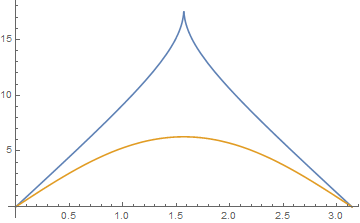
\includegraphics[scale=0.3]{perimeter.png} \caption{\small Functions $R\mapsto{\rm vol}(\partial D_R)$ and $R\mapsto2\pi \sin{R}$ for $R\in [0,\pi]$. }\label{fig:perimeter}
\end{figure}
In figure \ref{fig:perimeter} we have plotted the numerical computations made by Mathematica of the functions $R\mapsto {\rm vol}(\partial D_t)$ and $R\mapsto {\rm vol}\left(\partial B^{2,1}_R\right)=2\pi\sin(R)$.

In order to obtain the volume of the extrinsic balls we are going to use the following obvious coordinate system (chart) of the Clifford torus
$$
\varphi:(-\pi,\pi)\times(-\pi,\pi) \to \Sigma,\quad \varphi(\alpha,\beta)=\frac{1}{\sqrt{2}}\left(\cos(\alpha),\sin(\alpha),\cos(\beta),\sin(\beta)\right)
$$
Given two complex numbers $z_1,z_2\in \Sigma$, the coordinates functions with respect to the chart $\varphi$ are given by
$$
\varphi^{-1}(z_1,z_2)=\left({\rm arg}(z_1),{\rm arg}(z_2)\right)
$$
where here ${\rm arg}$ takes values in $(-\pi,\pi)$.  This particular chart  covers almost every point in $\Sigma$, indeed the set $\Sigma-\varphi\left((-\pi,\pi)\times (-\pi,\pi)\right)$ is just
$$
\left\{\frac{1}{\sqrt{2}}(-1,e^{i \theta})\, :\, \theta\in [-\pi,\pi]\right\}\cup\left\{\frac{1}{\sqrt{2}}(e^{i \theta},-1)\, :\, \theta\in [-\pi,\pi]\right\}.
$$
The co-ordinate vector fields $\{\frac{\partial}{\partial \alpha},\frac{\partial}{\partial \beta} \}$ are thus given by
$$
\frac{\partial }{\partial \alpha}=\frac{1}{\sqrt{2}}\left(-\sin\alpha,\, \cos\alpha,\, 0,\, 0\right),\quad \frac{\partial }{\partial \beta}=\frac{1}{\sqrt{2}}\left(0,\, 0,\, -\sin\beta,\, \cos\beta\right) 
$$
This vector fields can be extended to two smooth vectors fields on $\mathbb{C}^2$ given by
$$
\frac{\partial}{\partial \alpha}(z_1,z_2)=(iz_1,0),\quad \frac{\partial}{\partial \beta}(z_1,z_2)=(0,iz_2).
$$
The metric tensor can be expressed as
$$
g=\frac{1}{2}d\alpha\otimes d\alpha+\frac{1}{2}d\beta\otimes d\beta 
$$
with  Riemannian volume form given by
$$
\omega_g=\frac{1}{2}d\alpha\wedge d\beta=d\left(-\frac{1}{2}\beta d\alpha\right)=d\Omega
$$
where $\Omega=-\frac{1}{2}\beta d\alpha$. Therefore
$$
{\rm vol}(D_R(o))=\int_{D_R}\omega_g=\int_{\partial D_R} \Omega
$$
Hence, for $R<\frac{\pi}{2}$, 
$$
{\rm vol} (D_R(o))=\int_{-\arccos(2\cos(R)-1)}^{\arccos(2\cos(R)-1)}\arccos\left({2\cos(R)-\cos(t)}\right)dt.
$$
Similarly for $R>\frac{\pi}{2}$ we obtain
$$
{\rm vol} (D_R(o))=\int_{\arccos(2\cos(R)+1)}^{2\pi-\arccos(2\cos(R)+1)}\arccos\left({2\cos(R)-\cos(t)}\right)dt.
$$
\begin{figure}
    \centering
    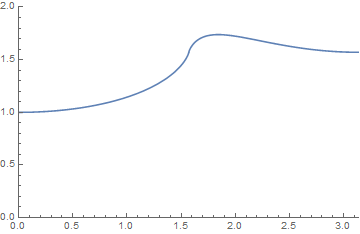
\includegraphics[scale=0.5]{vol.png}
    \caption{\small Numerical computations of $\frac{{\rm vol}(D_t(o))}{{\rm vol}\left(B^{2,1}_t\right)}$ for $t\in [0,\pi]$}\label{fig:volume}
\end{figure}
Numerical computations made by Mathematica for the quotient 
$$
t\mapsto \frac{{\rm vol}(D_t(o))}{{\rm vol}\left(B^{2,1}_t\right)}=\frac{{\rm vol}(D_t(o))}{2\pi(1-\cos(t))}
$$
are plotted in figure \ref{fig:volume}.






\section{Open problems}
In section \ref{Clifford} we have shown explicit computations and numerical evidences for the behavior of the function $$t\mapsto \frac{{\rm vol}(D_t(p))}{{\rm vol}\left(B^{2,1}_t\right)}$$ in the particular case of the Clifford torus. By theorem \ref{teounua} we know that this function can not   be always non-decreasing, neither always non-increasing in $(0, \pi)$.  The alluded numerical evidences (see figure \ref{fig:volume} ) suggest that this function is non-decreasing for $t\in (0,\pi/2)$. It is not clear for us if this is a particular behavior of the Clifford torus or the general case. Hence, we ask for the still open question
\begin{open}
Is the function 
$t\mapsto \frac{{\rm vol}(D_t(p))}{{\rm vol}\left(B^{n,1}_t\right)}$
non-decreasing for $t\in (0,\pi/2)$?
\end{open}
Moreover, We say that our monotonicity formula, given by theorem \ref{teodua}, 
\begin{equation}\label{lodemoatros}
\frac{{\rm vol}(D_{t_1}(o))-{\rm vol}\left(B^{n,1}_{t_1}\right)}{{\rm vol}\left( \partial B^{n,1+1}_{t_1}\right)}   \leq  \frac{{\rm vol}(D_{t_2}(o))-{\rm vol}\left(B^{n,1}_{t_2}\right)}{{\rm vol}\left( \partial B^{n,1+1}_{t_2}\right)} \quad {\rm for}\quad 0<t_1\leq t_2<\pi
\end{equation}
improves the monotonicity formula of \cite{Kokarev2021}, \emph{i.e},
\begin{equation}\label{lodeKoka}
\frac{{\rm vol}(D_{t_1}(o))}{{\rm vol}\left( \partial B^{n,1+1}_{t_1}\right)}   \leq  \frac{{\rm vol}(D_{t_2}(o))}{{\rm vol}\left( \partial B^{n,1+1}_{t_2}\right)} \quad {\rm for}\quad 0<t_1\leq t_2<\pi
\end{equation}
because inequality \eqref{lodemoatros} can not be deduced from \eqref{lodeKoka} but inequality \eqref{lodemoatros} implies inequality \eqref{lodeKoka}. A natural question is hence the following
\begin{open}
Can inequality \eqref{lodemoatros} be improved?
\end{open}

Following the example of the Clifford torus (shown in section \ref{Clifford}).  By the results of \cite{CLY1984} can be stated that 
$$
{\rm vol(\partial D_t(p)})\geq {\rm vol}\left(\partial B^{2,1}_t\right)
$$
for any $t\in (0,\pi/2)$. As we see, there is still a lack of information about the behavior of the volume of the extrinsic spheres with radius beyond $\frac{\pi}{2}$. In fact, we have, in the  example of the Clifford torus, numerical evidences with the volume of extrinsic spheres which suggest (see figure \ref{fig:perimeter}) that the function 
$$
t\mapsto {\rm vol(\partial D_t(p)})
$$
is not smooth in $t=\pi/2$ but 
$$
{\rm vol(\partial D_t(p)})\geq {\rm vol}\left(\partial B^{2,1}_t\right)
$$
for any $t$ in the whole interval $(0,\pi)$. We can ask thence
\begin{open}
Is 
$
{\rm vol(\partial D_t(p)})\geq {\rm vol}\left(\partial B^{n,1}_t\right)
$
for any $t\in (0,\pi)$?
\end{open}


%%%%%%%%%%%%%%%%%
%\subsection{Acknowledgement}\

%The authors  wish to thank...

\bibliographystyle{plain}
\bibliography{concentration}
 
\end{document}

